% Author: Seongjin Lee 
% Gyeongsang National University, Korea 
% 
% 2017-03-06
%

\documentclass[newPxFont,sthlmFooter,nooffset]{beamer}
\usepackage{kotex}
%\usetheme{sthlm}
\usepackage{../style/beamerthemesthlm}
\hypersetup{pdfauthor={Seongjin Lee (insight@gnu.ac.kr)},
            pdfsubject={Data Structure and Algorithm, Lecture Note},
            pdfkeywords={Data Structure, Algorithm, Lecture, Note},
            pdfmoddate={D: \pdfdate},
            pdfcreator={Seongjin Lee}}

%\setbeamertemplate{footline}[text line]{%
%    \parbox{\linewidth}{\vspace*{-8pt} \insertsectionhead  \hfill\insertshortauthor\hfill\insertpagenumber}}
%\setbeamertemplate{navigation symbols}{}


\setbeamertemplate{blocks}[rounded]

\title{Data Structure and Algorithm}
\subtitle{Class 3}
\author[SJL]{Seongjin Lee}
\institute{\href{mailto:insight@gnu.ac.kr}{insight@gnu.ac.kr}\\\url{http://resourceful.github.io}\\Systems Research Lab.\\GNU}
\date{2017-03-06} 

\begin{document}



\frame[plain,t]{\titlepage} 

\frame{\frametitle{Table of contents}\tableofcontents} 


%---------------------------------------------------------
\section{Array} 
\begin{frame}[t]
  \frametitle{Array}
an \textbf{array} is a set of pairs, \textbf{<index, value>}, such that each index that is defined has a value associated with it
\begin{itemize}
\item  ``a consecutive set of memory locations'' in C
\item  logical order is the same as physical order
\end{itemize}

operations
\begin{itemize}
\item creating a new array
\item retrieves a value
\item stores a value
\item insert a value into array - delete a value at the array
\end{itemize}

\end{frame}

\begin{frame}[t, fragile]
  \frametitle{Array}
A one-dimensional array in C is declared implicitly by appending brackets to the name of a variable

\begin{codedef}
  int list[5], *plist[5];
\end{codedef}

arrays start at index 0 in C  
\end{frame}

\begin{frame}[t, fragile]
  \frametitle{Array}
consider the implementation of one-dimensional arrays

\begin{codedefnb}
int list[5];
\end{codedefnb}

\begin{itemize}
\item allocates five consecutive memory locations
\item each memory location is large enough to hold a single integer
\item base address address of the first element
\end{itemize}

\begin{codedefnb}
list = &list[0]
\end{codedefnb}

\end{frame}


\begin{frame}[t, fragile]
  \frametitle{Array}
  
  \begin{tabular}{l  l}
    Variable & Memory Address \\ \hline
\texttt{\&list[0]} & base address = $\alpha$ \\
\texttt{\&list[1]} & $\alpha +$ \texttt{sizeof(int)}\\
\texttt{\&list[2]} & $\alpha + 2 \cdot$ \texttt{sizeof(int)}\\
\texttt{\&list[3]} & $\alpha + 3 \cdot$ \texttt{sizeof(int)}\\
\texttt{\&list[4]} & $\alpha + 4 \cdot$ \texttt{sizeof(int)}\\
  \end{tabular}

\bigskip
\texttt{\&list[i]} in a C programs
\begin{itemize}
\item C interprets it as a pointer to an integer or its value
\end{itemize}

\end{frame}

\begin{frame}[t, fragile]
  \frametitle{Array}
\begin{codedef}
int *list1;          // pointer variable to an int
\end{codedef}

\begin{codedef}
int *list2[5];       // list2 : pointer constant to an int, 
                     // and five memory locations for holding 
                     // integers are reserved
\end{codedef}

\texttt{(list2+i)} equals \texttt{\&list2[i]}, and \texttt{*(list2+i)} equals \texttt{list2[i]}
\begin{itemize}
\item regardless of the type of the array list2
\end{itemize}
\end{frame}

\begin{frame}[t]
  \frametitle{Array}
consider the way C treats an array when it is a parameter to a function
\begin{itemize}
\item the parameter passing is done using call-by-value in C
\item but array parameters have their values altered
\end{itemize}

\end{frame}

\begin{frame}[t, fragile]
  \frametitle{Array: Example 2.1}
\begin{codedef}
#define MAX_SIZE 100
float sum(float [], int); 
float input[MAX_SIZE], answer; 
int i;

void main(void) {
    for(i = 0; i < MAX_SIZE; i++) input[i] = i;
        answer = sum(input, MAX_SIZE);
    printf{"The sum is: %f\n", answer);
}     

float sum(float list[], inst n) {
    int i;
    float tempsum = 0;
    for(i = 0; i < n; i++)
        tempsum += list[i];
    return tempsum;
}
\end{codedef}
\end{frame}






\begin{frame}[t, fragile]
  \frametitle{Recap: On Pointer}
Pointer Variable stores address
\begin{itemize}
\item \& : Starting address of allocated variable
\item * : Value stored on the address of the pointer variable
\end{itemize}
\lstinputlisting[lineskip=1pt, numbers=left]{codes/pointer_variable.c}
\end{frame}



\begin{frame}[t, fragile]
  \frametitle{Recap: On Pointer}
Do Not!
  \begin{itemize}
  \item pointer variable is not referencing an address, so cannot store a value
\begin{codedef}
int *ptr;
* ptr = 100;
\end{codedef}
\item the data type must equal
\begin{codedef}
double Pi = 3.14;
int *pPi = &Pi; 
\end{codedef}
\item cannot dereference a non-pointer variable
\begin{codedef}
int num;
*num = 100;  
\end{codedef}
\item it is recommended to initialize a pointer value with NULL ('\textbackslash 0')
  \end{itemize}
\end{frame}


\begin{frame}[t, fragile]
  \frametitle{Recap: On Pointer}
Do!
  \begin{itemize}
\item it is recommended to initialize a pointer value with NULL ('\textbackslash 0') \\ 
See the example

  \end{itemize}
\end{frame}

\begin{frame}[t, fragile]
  \frametitle{Recap: On Pointer}
\begin{codedef}
#include <stdlib.h

void *malloc(size_t size); // allocates size bytes of memory and returns a pointer to the allocated memory
void *free(void *ptr); // frees allocation that were created via the preceding allocation function
void *calloc(size_t count, size_t size); // contiguously allocates enough sapce for count objects that are size bytes of memory each and returns a pointer to the allocated memory. The allocated memory is filled with bytes of value zero.
void *realloc(void *ptr, size_t size); // change the size of the allocation pointed to by ptr to size, and returns ptr
\end{codedef}

\end{frame}




\begin{frame}[t, fragile]
  \frametitle{Array: Ex 2.2, 1-dimensional array addressing}
\begin{codedef}
int one[] = {0, 1, 2, 3, 4};   
\end{codedef}

write a function that prints out both the address of the $i^{th}$ element of the array and the value found at this address

\end{frame}

\begin{frame}[t, fragile]
  \frametitle{Array:  Ex 2.2 One dimensional array accessed by address}

\lstinputlisting[lineskip=1pt]{codes/array_address.c}

One-dimensional array accessed by address
\begin{itemize}
\item address of \texttt{i} th element \texttt{ptr + i}
\item obtain the value of the \texttt{i} th value \texttt{*(ptr + i)}
\end{itemize}

\end{frame}

\begin{frame}[t, fragile]
  \frametitle{Array}
\begin{codedefnb}
Address		Contents
1518325632	    0
1518325633	    1
1518325634	    2
1518325635	    3
1518325636	    4
\end{codedefnb}
\bigskip
One-dimensional array addressing
\begin{itemize}
\item the addresses increase by two on an Intel 386 machine
\item Example shown is the result of Mac OS X on Intel Core i5 Machine
\end{itemize}

\end{frame}


\section{Structures and Unions}

\begin{frame}[t]
  \frametitle{Structures and Unions: struct}
\textbf{struct}  
\begin{itemize}
\item structure or record
\item the mechanism of grouping data
\item permits the data to vary in type
\end{itemize}
\bigskip

collection of data items where
\begin{itemize}
\item each item is identified as to its type and name
\end{itemize}

\end{frame}


\begin{frame}[t, fragile]
  \frametitle{Structures and Unions: struct}
\begin{codedef}
struct {
    char name[10];
    int age;
    float salary;
} person;
\end{codedef}
\bigskip
creating a variable
\begin{itemize}
\item whose name is person and
\item has three fields
  \begin{enumerate}
  \item a name that is a character array
  \item an integer value representing the age of the person
  \item a float value representing the salary of the individual
  \end{enumerate}

\end{itemize}

\end{frame}


\begin{frame}[t, fragile]
  \frametitle{Structures and Unions: struct}
use of the . as the structure member operator

\begin{codedef}
strcpy(person.name, "james");
person.age = 30;
person.salaray = 35000;  
\end{codedef}
\bigskip
\begin{itemize}
\item select a particular member of the structure
\end{itemize}

 
\end{frame}


\begin{frame}[t, fragile]
  \frametitle{Structures and Unions: struct}
\texttt{typedef statement}
\begin{itemize}
\item create our own structure data type
\end{itemize}

type 1
\begin{codedef}
typedef struct human_being { 
    char name[10];
    int age;
    float salary;
};
\end{codedef}

type 2
\begin{codedef}
typedef struct { 
    char name[10]; 
    int age;
    float salary;
} human_being;
\end{codedef}
\end{frame}


\begin{frame}[t, fragile]
  \frametitle{Structures and Unions: struct}
\texttt{human\_being}  
\begin{itemize}
\item the name of the type defined by the structure definition
\end{itemize}

\begin{codedef}
human_being person1, person2;

if(strcmp(person1.name, person2.name)) 
    printf("The two people do not have the same name\n");
else
    printf("The two people have the same name\n");
\end{codedef}
\end{frame}


\begin{frame}[t, fragile]
  \frametitle{Structures and Unions: Assignment}
\textbf{assignment}
\begin{itemize}
\item permits structure assignment in ANSI C

\begin{codedef}
  person1 = person2;
\end{codedef}
\item but, in most earlier versions of C assignment of structures is not permitted
\begin{codedef}
   strcpy(person1.name,person2.name); 
   person1.age=person2.age; 
   person1.salary=person2.salary;    
\end{codedef}
\end{itemize}
\end{frame}


\begin{frame}[t, fragile]
  \frametitle{Structures and Unions: Equality or Inequality}
\textbf{equality or inequality}
\begin{itemize}
\item cannot be directly checked
\item Example function to check equality of struct
\begin{codedef}
int humans_equal(human_being person1, human_being person2) { 
    if(strcmp(person1.name,person2.name))
        return FALSE; 
    if(person1.age!=person2.age)
        return FALSE; 
    if(person1.salary!=person2.salary)
        return FALSE; 
    return TRUE;
}    
\end{codedef}
\end{itemize}

\end{frame}


\begin{frame}[t, fragile]
  \frametitle{Structures and Unions: Embedding Structure}
Embedding of a structure within a structure
\begin{codedef}
typedef struct { 
    int month; 
    int day;
    int year;
} date;

typedef struct human_being { 
    char name[10];
    int age;
    float salary;
    date dob; // embedded structure
};  
\end{codedef}
\end{frame}

\begin{frame}[t, fragile]
  \frametitle{Structures and Unions: Embedding Structure}
Ex. A person boar on Feb 14 1992
\begin{codedef}
person1.dob.month = 2;
person1.dob.day = 14;
person1.dob.year = 1992;
\end{codedef}
\end{frame}


\begin{frame}[t]
  \frametitle{Structures and Unions: Unions}
\textbf{Unions}
\begin{itemize}
\item similar to a structure, but
\item the fields of a union must share their memory space
\item only one field of the union is ``active'' at any given time
\end{itemize}
\end{frame}

\begin{frame}[t, fragile]
  \frametitle{Structures and Unions: Unions}
\begin{codedef}
typedef struct sex_type {
    enum tag_field {female,male} sex; 
    union {
        int children;
        int beard; } u;
};

typedef struct human_being {
    char name[10]; 
    int age;
    float salary; 
    date dob; 
    sex_type sex_info;
};

human_being person1,person2;    
\end{codedef}
\end{frame}

\begin{frame}[t, fragile]
  \frametitle{Structures and Unions: Unions}
Assign values to \texttt{person1} and \texttt{person2}
\begin{codedef}
persone1.sex_info.sex = male; 
person1.sex_info.u.beard = FALSE; /* FALSE: 0 */
\end{codedef}

and

\begin{codedef}
person2.sex_info.sex = female; 
person2.sex_info.u.children = 4;
\end{codedef}
\end{frame}

\begin{frame}[t, fragile]
  \frametitle{Structures and Unions: {\large Internal Implementation of Structure}}
\begin{codedef}
struct {
    int i, j; float a, b;
}  
\end{codedef}

or 
\begin{codedef}
struct {
    int i; int j; float a; float b;
};
\end{codedef}
\bigskip
stored in the same way
\begin{itemize}
\item increasing address locations in the order specified in the
  structure definition
\end{itemize}

size of an object of a struct or union type
\begin{itemize}
\item the amount of storage necessary to represent the largest
  component
\end{itemize}

\end{frame}

\begin{frame}[t, fragile]
  \frametitle{Structures and Unions: {\large Self-referential structures}}
  \begin{itemize}
  \item one or more of its components is a pointer to itself
  \item usually require dynamic storage management routines to
    explicitly obtain and release memory
  \end{itemize}
\begin{codedef}
typedef struct list {
    char data;
    list *link;
};    
\end{codedef}
the value of \texttt{link}
\begin{itemize}
\item address in memory of an instance of \texttt{list} or \texttt{null} pointer
\end{itemize}
\end{frame}

\begin{frame}[t, fragile]
  \frametitle{Structures and Unions: {\large Self-referential structures}}
\begin{codedef}
list item1, item2, item3;
item1.data = 'a';
item2.data = 'b';
item3.data = 'c';
item1.link = item2.link = item3.link = NULL;   
\end{codedef}
\begin{uncoverenv}<2->
attach these structures together
\begin{codedef}
item1.link = &item2;
item2.link = &item3;
\end{codedef}
\end{uncoverenv}
\end{frame}





\section{Sparse Matrices}

\begin{frame}[t, fragile]
  \frametitle{The Sparse Matrix: {\large representing matrix by using array}}
  \begin{itemize}
  \item $m$ by $n$ ($m$ rows, $n$ columns)
  \item use two-dimensional array
  \item space complexity \\
        $S(m, n) = m *n$
  \end{itemize}

\begin{equation*}
  \begin{blockarray}{r *{3}{c}}
      & col0 & col1 & col2 \\
\begin{block}{l [*{3}{c}]}
 row0 & -27  &   3  &  4   \\
 row1 &   6  &  82  &  -2  \\
 row2 & 109  & -64  &  11   \\
 row3 &  12  &   8  &  9   \\
 row4 &  48  &  27  & 47   \\
\end{block}
  \end{blockarray}
\end{equation*}
\end{frame}

\begin{frame}[t, fragile]
  \frametitle{The Sparse Matrix}
\texttt{A[6,6]}

\begin{equation*}
  \begin{blockarray}{r *{6}{c}}
      & col0 & col1 & col2 & col3 & col4 & col5 \\
\begin{block}{l [*{6}{c}]}
 row0 & 15  & 0   & 0  &  22 &   0 &   15   \\
 row1 & 0   & 11  & 3  &   0 &   0 &   0   \\
 row2 & 0   & 0   & 0  &  -6 &   0 &   0   \\
 row3 & 0   & 0   & 0  &   0 &   0 &   0   \\
 row4 & 91  & 0   & 0  &   0 &   0 &   0   \\
 row5 & 0   & 0   & 28 &   0 &   0 &   0   \\
\end{block}
  \end{blockarray}
\end{equation*}
\end{frame}

\begin{frame}[t, fragile]
  \frametitle{The Sparse Matrix}
common characteristics
\begin{itemize}
\item most elements are zero's 
\item inefficient memory utilization
\end{itemize}
\bigskip

solutions
\begin{itemize}
\item store only nonzero elements
\item using the triple \texttt{<row,col,value>}
\item must know
  \begin{itemize}
  \item the number of rows
  \item the number of columns
  \item the number of non-zero elements
  \end{itemize}

\end{itemize}

\end{frame}

\begin{frame}[t, fragile]
  \frametitle{The Sparse Matrix}
\begin{codedef}
#define MAX_TERMS 101 

typedef struct {
    int col; 
    int row; 
    int value;
} term;

term a[MAX_TERMS];  
\end{codedef}
\begin{itemize}
\item a[0].row: the number of rows
\item a[0].col: the number of columns
\item a[0].value: the total number of non-zoros
\item choose row-major order
\end{itemize}
\end{frame}

\begin{frame}[t, fragile]
  \frametitle{The Sparse Matrix: As Tripels}
  \begin{center}
    \begin{tabular}{r c c c}
      & row & col & value \\ \hline
      a[0]&  6  &  6  &   8   \\
      a[1]&  0  &  0  &  15   \\ 
      a[2]&  0  &  3  &  22   \\ 
      a[3]&  0  &  5  & -15   \\ 
      a[4]&  1  &  1  &  11   \\ 
      a[5]&  1  &  2  &   3   \\ 
      a[6]&  2  &  3  &  -6   \\ 
      a[7]&  4  &  0  &  91   \\ 
      a[8]&  5  &  2  &  28   \\ 
    \end{tabular}
  \end{center}
  \begin{itemize}
  \item space complexity (*variable space requirement) \\
\texttt{S(m,n) = 3 * t} where \\
\texttt{t} : the number of non-zero’s
\item independent of the size of rows and columns
  \end{itemize}

\end{frame}

\begin{frame}[t, fragile]
  \frametitle{The Sparse Matrix: Transpose}
Transpose a matrix
\begin{itemize}
\item interchange rows and columns
\item move \texttt{a[i][j]} to \texttt{a[j][i]}
\end{itemize}
  \begin{center}
    \begin{tabular}{r c c c}
      & row & col & value \\ \hline
      b[0]&  6  &  6  &   8   \\
      b[1]&  0  &  0  &  15   \\ 
      b[2]&  0  &  4  &  91   \\ 
      b[3]&  1  &  1  &  11   \\ 
      b[4]&  2  &  1  &   3   \\ 
      b[5]&  2  &  5  &  28   \\ 
      b[6]&  3  &  0  &  22   \\ 
      b[7]&  3  &  2  &  -6   \\ 
      b[8]&  5  &  0  &  -15   \\ 
    \end{tabular}
  \end{center}
\end{frame}

\begin{frame}[t, fragile]
  \frametitle{The Sparse Matrix}
\begin{codedef}
algorithm BAD_TRANS 
for each row i
    take element <i,j,value>;
    store it as element <j,i,value> of the transpose; 
end;  
\end{codedef}
The problem
\begin{itemize}
\item <2-> data movement
\end{itemize}
\begin{uncoverenv}<3->
\begin{codedef}
algorithm TRANS
for all elements in column j
    place element <i,j,value> in element <j,i,value> end;
\end{codedef}
The problem
\end{uncoverenv}
\begin{itemize}
\item <4-> unnecessary loop for each column
\end{itemize}
\end{frame}


\begin{frame}[t, fragile]
  \frametitle{The Sparse Matrix: Transpose}
\begin{codedef}
void transpose(term a[], term b[]) {
    int n, i, j, currentb;
    n = a[0].value; 
    b[0].row = a[0].col;
    b[0].col = a[0].row; 
    b[0].value = n;
    if(n > 0){
        currentb = 1;
        for (i = 0; i < a[0].col; i++)
            for(j = 1; j <= n; j++)
                if(a[j].col == i) {
                  b[currentb].row = a[j].col;  
                  b[currentb].col = a[j].row;  
                  b[currentb].value = a[j].valuel;  
                  cuurentb++;
            }
    }
}
\end{codedef}
Space and Time complexity?
\end{frame}

\begin{frame}[t, fragile]
  \frametitle{The Sparse Matrix: Transpose}
\textbf{Complexity}
\begin{itemize}
\item space: 3$\times$ t
\item time: O(cols$\times$ t)
\end{itemize}

create better algorithm by using a little more storage
\begin{itemize}
\item row\_terms the number of element in each row
\item starting\_pos the starting point of each row
\end{itemize}

\end{frame}

\begin{frame}[t, fragile, allowframebreaks]
  \frametitle{The Sparse Matrix: Better Transpose}
\begin{codedef}
void fast_transpose(term a[], term b[]){
    int row_terms[MAX_COL];
    int starting_pos[MAX_COL];
    
    int i, j;
    
    int num_cols = b[0].row = a[0].col;
    int num_terms = b[0].value = a[0].value;

    b[0].col = a[0].row;

    if(num_terms > 0) {
        for(i = 0; i < num_cols; i++)
            row_terms[i] = 0;

        for(i = 1; i <= num_terms; i++)
            row_terms[a[i].col]++;

        starting_pos[0] = 1;

        for(i = 1; i < num_cols; i++)
            starting_pos[i] = starting_pos[i-1] + row_terms[i-1];

        for(i = 1; i <= num_terms; i++){
            j = starting_pos[a[i].col]++;
            b[j].row = a[i].col;
            b[j].col = a[i].row;
            b[j].value = a[i].value;
        }
    }
}  
\end{codedef}
\end{frame}

\begin{frame}[t, fragile]
  \frametitle{The Sparse Matrix: Better Transpose}
  \begin{tabular}{r  *{6}{c}}
    & [0] & [1] & [2] & [3] & [4] & [5] \\
row\_terms= & 2 & 1 & 2 & 2 & 0 & 1 \\
starting\_pos= & 1 & 3 & 4 & 6 & 8 & 8\\
  \end{tabular}

\textbf{complexity}
\begin{itemize}
\item space: 3$\times$ t + extra
\item time: O(cols + t)
\end{itemize}
\end{frame}

\section{Representation of Multidimensional Arrays}



\begin{frame}[t, fragile]
  \frametitle{Representation of Multidimensional Arrays}
internal representation of multidimensional arrays
\begin{itemize}
\item how to state n-dimensional array into 1-dimensional array ?
\item how to retrieve arbitrary element in an array
\texttt{  a[upper$^0$][upper$^1$] $\cdots$ [upper$^{n-1}$]}
\end{itemize}

The number of elements in the array
$\prod ^{n-1}_{i=0} upper^{i}$

Ex. a[10][10][10]
\begin{itemize}
\item $10\times 10 \times 10 = 1000$ (units)
\end{itemize}
\end{frame}


\begin{frame}[t, fragile]
  \frametitle{Representation of Multidimensional Arrays}
represent multidimensional array by
\begin{itemize}
\item in what order ?
\end{itemize}


\textbf{row-major-order}
\begin{itemize}
\item store multidimensional array by rows
\end{itemize}
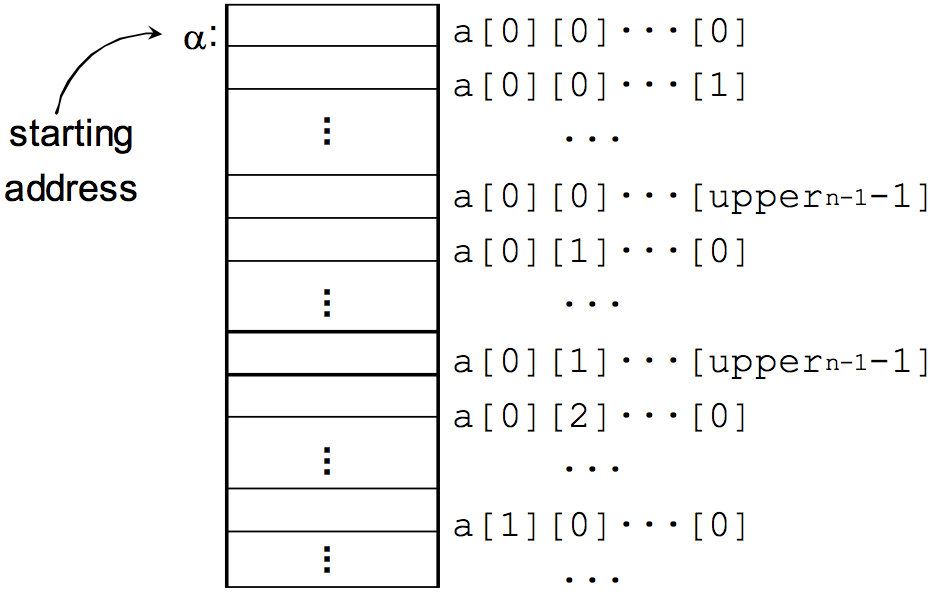
\includegraphics[width=0.7\textwidth]{figures/fig01_multi_dim.png}
\end{frame}


\begin{frame}[t, fragile]
  \frametitle{Representation of Multidimensional Arrays}
how to retreive values
\begin{itemize}
\item starting-address + offset-value
\item assume α: starting-address
\end{itemize}

\textbf{1-dimensional} array \texttt{a[u$^0$]}

\begin{center}
  \begin{tabular}{r r} \hline
    \&a[0] & : $\alpha$ \\
    \&a[1] & : $\alpha + 1$ \\[-0.5em]
    $\cdot$ & $\cdot$ \\[-0.5em]
    $\cdot$ & $\cdot$ \\[-0.5em]
    $\cdot$ & $\cdot$ \\
    \&a[u$^0$-1] & : $\alpha + (u^0 -1)$ \\ \hline
    \&a[i] & : $\alpha + i$ \\
  \end{tabular}
\end{center}
\end{frame}


\begin{frame}[t, fragile]
  \frametitle{Representation of Multidimensional Arrays}
\textbf{2-dimensional} array \texttt{a[u$^0$][u$^1$]}

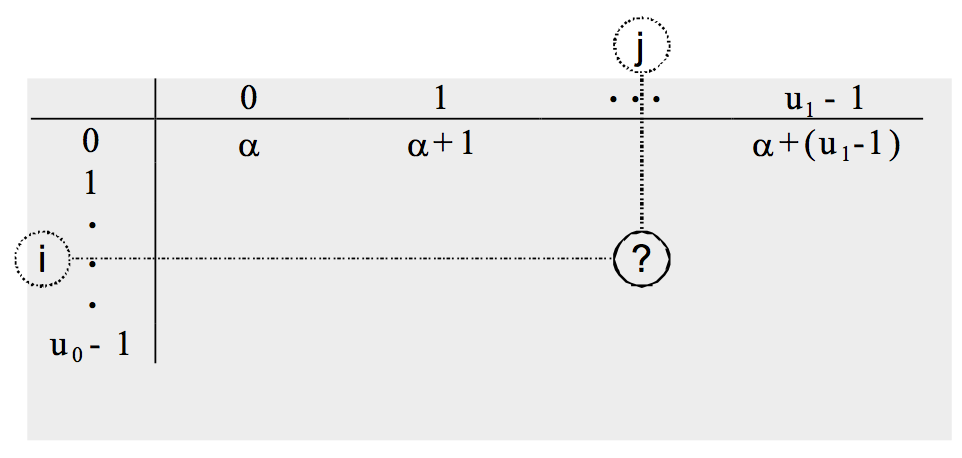
\includegraphics[width=0.7\textwidth]{figures/fig02_2-dim_array.png}

\texttt{\&a[i][j] =} $\alpha+i\cdot u^1 + j$
\end{frame}


\begin{frame}[t, fragile]
  \frametitle{Representation of Multidimensional Arrays}
\textbf{2-dimensional} array \texttt{a[u$^0$][u$^1$][u$^2$]}
\begin{eqnarray*}
\&a[i][j][k] &=& \alpha + i\cdot u^1 \cdot u^2 + j\cdot u^2 +k \\
             &=& \alpha + u^2[i \cdot u^1 + j] +k
\end{eqnarray*}

\texttt{general} case array \texttt{a[u$^0$][u$^1$] $cdots$[u$^{n-1}$}

$\&a[i_0][i_1][i_{n-1}]$
\begin{equation*}
  = \alpha + \sum^{n-1}_{j=0} i_j \cdot a_j
  \begin{cases}
    a_j = \prod^{n-1}_{k=j+1} u_k & \text{for} ~j < n-1\\
    a_{n-1} = 1 & \text{for} ~j = n-1
  \end{cases}
\end{equation*}
\end{frame}


\begin{frame}[t, fragile]
  \frametitle{Representation of Multidimensional Arrays}

\end{frame}









\end{document}
